\subsubsection{GUI}

Programmet QT blev anvendt til at designe og implementer brugergrænsefladen. Dette gave nogle udfordringer. Udfordringerne bestod primært i at kendskabet til programmet QT ikke var særligt stort. Da QT selv skaber klasserne og metoderne er det svært at beskrive disse på forhånd. Derfor blev det besluttet at klasserne først skulle udarbejdes efter at brugergrænsefladen var designet.

Det endelige klassediagram der blev udarbejdet kan ses illustreret på figur \ref{kd}. Dette klassediagram indeholder 5 forskellige klasser.

\centerline{\includegraphics[scale=1]{tex/Design/GUI/Fotos/Tom_klassediagram}}
	\caption{Klasserne indsættes i et klassediagram}}
	\label{kd}

Her kan det ses at der er oprettet to forskellige klasser til read og write funktionerne, som sørger for kommunikationen med PSoC. Der er oprettet en virtuel read og write, og en reel read og write. Den virtuelle er blot oprettet for at gøre det muligt at teste systemet før det endelige system er fuldt udviklet, mens den reelle klasse er oprettet til at bruges når det endelige system udvikles.

For at holde styr på den indtastede og den resterende tid er der blev oprettet en Count klasse . Denne count klasse er implementeret som en domainklasse da det er her den resterende tid for vinåbningen gemmes. Det er denne klasse som skal sørge for at tiden tælles ned når den startes. Illustrationen af countklassen kan ses på figur \ref{CT_CD}.

\begin{figure}[H]
	\centerline{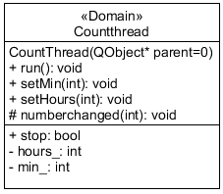
\includegraphics[scale=1]{tex/Design/GUI/Fotos/CountThread}}
	\caption{CountThread klasse illustreret}
	\label{CT_CD}
\end{figure}

Der er i alt 2 klasser i brugergrænsefladen. Der er en klasse for MainWindow, hvor alle funktionerne er defineret. MainWindow er klassen som sørger for at vise den grafiske brugergrænseflade. Det er her alle trykknap funktionerne er defineret. Klassen ses illustreret på figur \ref{MW_CD}. 

\begin{figure}[H]
	\centerline{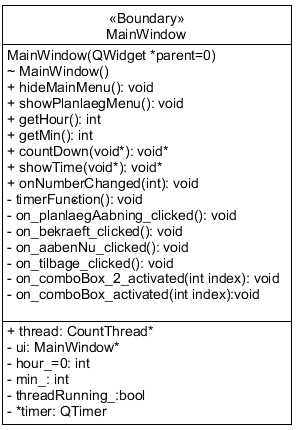
\includegraphics[scale=1]{tex/Design/GUI/Fotos/MainWindow}}
	\caption{MainWindow klasse illustreret}
	\label{MW_CD}
\end{figure}

For at se hele klasse diagrammet med alle metoder henvises der til bilag x.

Brugergrænsefladen er state styret. Derfor har det været nødvendigt at lave et statemachine diagram for brugergrænsefladen. Statemachinen ses på figur \ref{sm}\\

\centerline{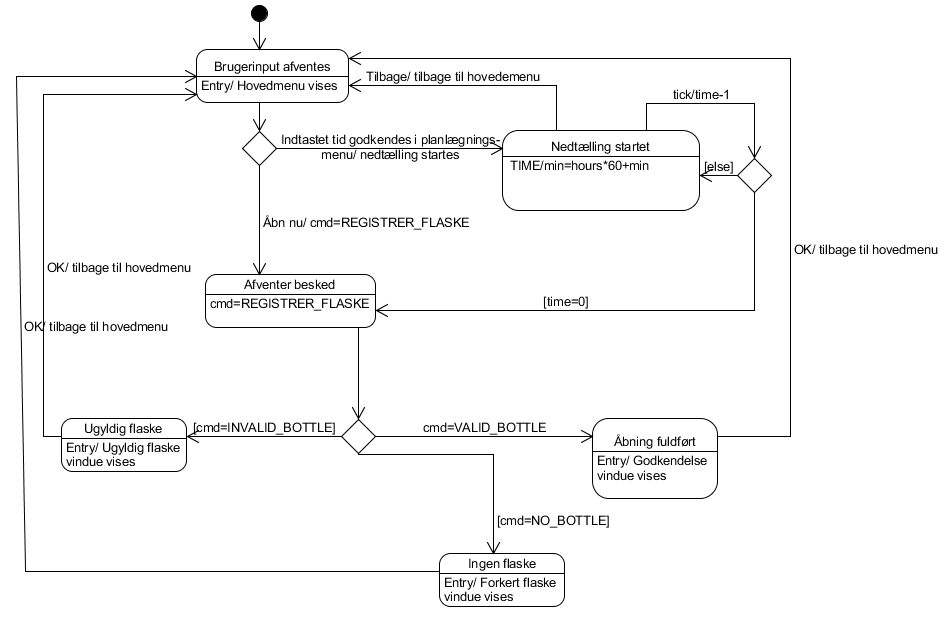
\includegraphics[scale=1]{tex/Design/GUI/Fotos/sm}}
	\caption{statemachine}
	\label{sm}

som illustreret i figuren starter systemet i en state der hedder "Brugerinput afventes". Denne state beskriver systemet når, brugergrænsefladen er i hovedmenuen. Her kan brugeren gøre 2 ting. Enten trykke på "Åbn nu" og få vinen åbnet med det samme, eller trykke på planlæg åbning, indtaste et åbningstidspunkt, for derefter at få systemet til at tælle ned til åbningstidpunktet. Vælger brugeren planlægningsmenuen, kan brugeren selvfølgelig navigere i systemet imens der bliver talt ned. Derfor er der ført en pil tilbage til "Brugerinput afventes". Når timeren sættes i gang, begynder den at tælle et minut ned ad gangen. Når minut og time antallet til sammen går ned på 0 bryder systemet ud af denne state og ind i en ny state der hedder "Afventer besked". I denne state ventes der på en besked fra PSoC'en. PSoC'en kan komme med 3 forskellige beskeder. Den første er at der ingen flaske er i systemet. Dette vil udløse et advarselsvindue på brugergrænsefladen. Den anden besked er at den indsatte flaske er ugyldig, hvilket også vil udløse et advarselsvindue. Den sidste besked man kan få er at flasken godkendes. Alle disse states fører brugeren tilbage til hovedmenuen ved at brugeren trykker OK på vinduet.
